\chapter{Django模型(数据库)}

\section{Django模型简介}
Django 对各种数据库提供了很好的支持，包括：PostgreSQL、MySQL、SQLite、Oracle。

Django 为这些数据库提供了统一的调用API。 我们可以根据自己业务需求选择不同的数据库。


\section{数据库的配置}
\subsection{sqlite3数据库配置}
Django 默认使用的是sqlite3数据库，不需要配置，也不需要安装额外的数据库驱动。
\subsubsection{settings.py配置}
\begin{lstlisting}[style=demostyle,numbers=none]
$> cd 主项目目录
$> cat settings.py
DATABASES = {
    'default': {
        'ENGINE': 'django.db.backends.sqlite3',
        'NAME': os.path.join(BASE_DIR, 'db.sqlite3'),
    }
}
\end{lstlisting}    

\subsection{MySQL数据库配置}
\subsubsection{安装MySQL驱动}
\begin{lstlisting}[style=demostyle,numbers=none]
$> sudo pip3 install pymysql
$> conda install pymysql
\end{lstlisting}

如果使用\codeinline{pymysql}需要在 \textcolor{YBXPurple}{主项目}的\codeinline{\_\_init\_\_.py}文件中添加如下代码：
\begin{lstlisting}[style=demostyle,numbers=none]
import pymysql
pymysql.install_as_MySQLdb()
\end{lstlisting}    

\subsubsection{提前配置数据库}
\textcolor{red}{\textbf{ORM 无法操作到数据库级别，只能操作到数据表}}
\begin{enumerate}[label=\arabic*)]
    \item 创建一个新数据库
\begin{lstlisting}[style=demostyle,numbers=none]
$> mysql -u root -p
mysql> create database 数据库名称 default charset=utf8; # 防止编码问题，指定为 utf8
\end{lstlisting}

    \item 创建一个新用户, 并授权(刷新权限)
\begin{lstlisting}[style=demostyle,numbers=none]
mysql> create user '用户名'@'主机名' identified by '密码'; # 主机名可以是 localhost
mysql> grant all privileges on 数据库名.* to '用户名'@'主机名'; # 授权
mysql> flush privileges; # 刷新权限
\end{lstlisting}

\end{enumerate}

\begin{example}
    \exProblem
    创建一个数据库\codeinline{django\_db}，用户名\codeinline{django\_user}，密码\codeinline{your\_password}，并授权\codeinline{django\_user}可以访问\codeinline{django\_db}数据库。
    \exSolution
\begin{lstlisting}[style=demostyle,numbers=none]
mysql> # 创建数据库    
mysql> CREATE DATABASE django_db DEFAULT CHARACTER SET utf8; 
Query OK, 1 row affected (0.03 sec)

mysql> # 创建用户
mysql> CREATE USER 'django_user'@'%' IDENTIFIED BY 'your_password';
Query OK, 1 row affected (0.03 sec)

mysql> # 授予 django_user，使其可以访问 django_db 数据库：
mysql> GRANT ALL PRIVILEGES ON django_db.* TO 'django_user'@'%';
Query OK, 0 rows affected (0.01 sec)

mysql> # 刷新权限
mysql> flush privileges;
Query OK, 0 rows affected (0.01 sec)
\end{lstlisting}
\end{example}


\subsubsection{配置settings.py}
\begin{lstlisting}[style=demostyle,numbers=none]
$> cat settings.py    
DATABASES = {
    'default': {
        'ENGINE': 'django.db.backends.mysql',
        'NAME': '数据库名称',
        'USER': '数据库用户名',
        'PASSWORD': '数据库密码',
        'HOST': '数据库地址',
        'PORT': '数据库端口',
    }
}
\end{lstlisting}


\begin{example}
    \exProblem
    配置MySQL数据库
    \exSolution
\begin{lstlisting}[style=demostyle,numbers=none]
$> cat settings.py    
DATABASES = {
    'default': {
        # 使用 MySQL 引擎
        'ENGINE': 'django.db.backends.mysql',  
        # 数据库名称，修改为你在 MySQL 中创建的数据库名
        'NAME': 'django_db',                   
        # 在 MySQL 中创建的用户名
        'USER': 'django_user',                 
        # 该用户的密码
        'PASSWORD': 'your_password',           
        # 如果 MySQL 在本地机器上，使用 localhost，或者是容器 IP
        'HOST': 'localhost',                   
        # MySQL 端口
        'PORT': '3306',                        
    }
}

# 运行数据库迁移
$> python manage.py migrate
Operations to perform:
  Apply all migrations: TestModel, admin, auth, contenttypes, jobs, sessions
Running migrations:
  Applying TestModel.0001_initial... OK
  Applying TestModel.0002_auto_20241114_0739... OK
  Applying TestModel.0003_auto_20241114_0804... OK
  Applying contenttypes.0001_initial... OK
  Applying auth.0001_initial... OK
  Applying admin.0001_initial... OK
  Applying admin.0002_logentry_remove_auto_add... OK
  Applying admin.0003_logentry_add_action_flag_choices... OK
  Applying contenttypes.0002_remove_content_type_name... OK
  Applying auth.0002_alter_permission_name_max_length... OK
  Applying auth.0003_alter_user_email_max_length... OK
  Applying auth.0004_alter_user_username_opts... OK
  Applying auth.0005_alter_user_last_login_null... OK
  Applying auth.0006_require_contenttypes_0002... OK
  Applying auth.0007_alter_validators_add_error_messages... OK
  Applying auth.0008_alter_user_username_max_length... OK
  Applying auth.0009_alter_user_last_name_max_length... OK
  Applying auth.0010_alter_group_name_max_length... OK
  Applying auth.0011_update_proxy_permissions... OK
  Applying jobs.0001_initial... OK
  Applying sessions.0001_initial... OK


# 查看数据库
$> docker start mysql57
$> docker exec -it mysql57 mysql -u root -p
Enter password:
mysql> show databases;
+--------------------+
| Database           |
+--------------------+
| information_schema |
| django_db          |
| mysql              |
| performance_schema |
| sys                |
| testdb             |
| testdb1            |
+--------------------+
7 rows in set (0.00 sec)

mysql> USE django_db;
Reading table information for completion of table and column names
You can turn off this feature to get a quicker startup with -A

Database changed
mysql> SHOW TABLES;
+----------------------------+
| Tables_in_django_db        |
+----------------------------+
| auth_group                 |
| auth_group_permissions     |
| auth_permission            |
| auth_user                  |
| auth_user_groups           |
| auth_user_user_permissions |
| django_admin_log           |
| django_content_type        |
| django_migrations          |
| django_session             |
| jobs                       |
| jobs_job                   |
| people                     |
+----------------------------+
13 rows in set (0.00 sec)

mysql>
\end{lstlisting}
\end{example}

\subsection{PostgreSQL数据库配置}
\subsubsection{安装psycopg2}
\begin{lstlisting}[style=demostyle,numbers=none]
$> sudo sh -c 'echo "deb http://apt.postgresql.org/pub/repos/apt $(lsb_release -cs)-pgdg main" > /etc/apt/sources.list.d/pgdg.list'
$> wget --quiet -O - https://www.postgresql.org/media/keys/ACCC4CF8.asc | sudo apt-key add -
$> sudo apt update
$> sudo apt install postgresql-server-dev-9.6
$> pg_config --version
PostgreSQL 9.6.24
$> pip install psycopg2==2.8.6 # 因为是Django3.X，所以安装2.8.6版本
\end{lstlisting}

或者安装预编译的二进制文件psycopg2-binary
\begin{lstlisting}[style=demostyle,numbers=none]
$> pip install psycopg2-binary
\end{lstlisting}

\subsubsection{[可选]配置 PostgreSQL 的远程访问}
默认情况下，PostgreSQL 仅允许本地访问。如果需要从其他容器或主机访问数据库，修改以下配置：
\begin{enumerate}[label=\arabic*)]
    \item 拷贝文件进行修改

\begin{lstlisting}[style=demostyle,numbers=none]
$> docker ps 
CONTAINER ID   IMAGE          COMMAND         NAMES
fcca6d8e3b95   postgres:9.6   "docker-ent…"   postgres96

$> docker exec postgres96 cp /var/lib/postgresql/data/pg_hba.conf /var/lib/postgresql/data/pg_hba.conf.bak
$> docker cp postgres96:/var/lib/postgresql/data/pg_hba.conf ./pg_hba.conf
$> vim pg_hba.conf
# 添加下面内容
host    django_db    django_user    0.0.0.0/0    md5

$> # 其中 host表示允许通过 TCP/IP 协议进行远程访问，而不是本地 Unix 套接字连接(local)。
$> # django_db 是数据库名称，django_user 是数据库用户名，
$> # 0.0.0.0/0 表示允许从任何 IP 地址访问。
$> # md5 表示使用 md5 加密方式验证密码。

$> docker cp ./pg_hba.conf postgres96:/var/lib/postgresql/data/pg_hba.conf
$> docker restart postgres96
\end{lstlisting}

    \item 直接\codeinline{echo}修改
\begin{lstlisting}[style=demostyle,numbers=none]
$> docker exec postgres96 cp /var/lib/postgresql/data/pg_hba.conf /var/lib/postgresql/data/pg_hba.conf.bak
$> docker exec postgres96 bash -c "echo 'host    django_db    django_user    0.0.0.0/0    md5' >> /var/lib/postgresql/data/pg_hba.conf"
$> docker restart postgres96
\end{lstlisting}        
\end{enumerate}

测试连接
\begin{lstlisting}[style=demostyle,numbers=none]
$> docker exec -it postgres96 psql -h localhost -U django_user -d django_db
\end{lstlisting}


\subsubsection{配置settings.py}
\begin{lstlisting}[style=demostyle,numbers=none]
$> cat settings.py    
DATABASES = {
    'default': {
        'ENGINE': 'django.db.backends.postgresql',
        'NAME': 'your_db',          # 数据库名称（默认为 postgres）
        'USER': 'your_user',        # 数据库用户（默认为 postgres）
        'PASSWORD': 'your_password',# 数据库密码
        'HOST': 'localhost',        # 主机地址
        'PORT': '5432',             # 端口号
    }
}
\end{lstlisting}

\begin{example}
    \exProblem
    创建一个数据库\codeinline{django\_db}，用户名\codeinline{django\_user}，密码\codeinline{django\_password}，
    并授权\codeinline{django\_user}可以访问\codeinline{django\_db}数据库。

    \exSolution
\begin{lstlisting}[style=demostyle,numbers=none]
$> $ docker exec -it postgres96 psql -U postgres
psql (9.6.24)
Type "help" for help.

postgres=# CREATE USER django_user WITH PASSWORD 'django_passwd';
CREATE ROLE

postgres=# CREATE DATABASE django_db OWNER django_user;
CREATE DATABASE

postgres=# GRANT ALL PRIVILEGES ON DATABASE django_db TO django_user;
GRANT
\end{lstlisting}

\begin{lstlisting}[style=demostyle,numbers=none]
$> docker restart postgres96
\end{lstlisting}

\begin{lstlisting}[style=demostyle,numbers=none]
$> cat settings.py
DATABASES = {
    'default': {
        'ENGINE': 'django.db.backends.postgresql',
        'NAME': 'django_db',          # 数据库名称
        'USER': 'django_user',        # 数据库用户名
        'PASSWORD': 'django_passwd',  # 数据库密码
        'HOST': 'localhost',          # 数据库主机
        'PORT': '5432',               # 数据库端口
    }
}
\end{lstlisting}    

运行数据库迁移
\begin{lstlisting}[style=demostyle,numbers=none]
$> python manage.py makemigrations
$> python manage.py migrate
\end{lstlisting}



    
\end{example}


\subsection{Redis数据库配置}

\section{定义模型}
\subsection{前提准备————创建子应用}
Django 规定，如果要使用模型，必须要创建一个子应用app。
\begin{lstlisting}[style=demostyle,numbers=none]
$> python manage.py startapp APP名
# 或者
$> django-admin startapp APP名
\end{lstlisting}

创建好了子应用后，会在项目目录下生成一个子应用目录，目录结构如下：
\begin{lstlisting}[style=demostyle,numbers=none]
$> django-admin startapp TestModel
$> $ tree TestModel/
TestModel/
|-- admin.py # 管理后台,
|-- apps.py # 应用配置
|-- __init__.py # 一个空文件，告诉 Python 该目录是一个 Python 包
|-- migrations  # 数据库迁移文件
│   `-- __init__.py
|-- models.py   # 模型文件
|-- tests.py    # 测试文件
`-- views.py    # 视图文件
\end{lstlisting}

\subsection{定义表结构}
\begin{enumerate}[label=\arabic*)]
    \item Django 的模型类必须继承自 \codeinline{django.db.models.Model} 类。

    \codeinline{models.Model} 是 Django 中定义模型类的基类，它包含了一些基本的属性和方法，用于定义数据库表的结构。

    \item 要在 \textcolor{YBXPurple}{子应用} 目录下的 \codeinline{models.py} 文件中定义模型类。
\end{enumerate}


\begin{lstlisting}[style=demostyle,numbers=none]
$> cat TestModel/models.py
from django.db import models # 导入模型类
 
"""
1.类名 People 表示数据库表名 
2.类属性 name 表示数据库表的字段名
  类属性 age 表示数据库表的字段名
3.类属性的值表示字段的类型
  CharField: 字符串类型 varchar
  IntegerField: 整数类型 int  
  max_length: 字符串类型的长度
"""
class People(models.Model):
    # id 在 Django 中会自动生成，不需要定义
    # id = models.AutoField(primary_key=True)
    name = models.CharField(max_length=20) # 相当于 varchar(20)
    age = models.IntegerField()
    gender = models.BooleanField(default=True)    
    # 外键关联，当关联的数据被删除时，本表中的数据也会被删除
    marjor = models.ForeignKey('Jobs', on_delete=models.CASCADE)

class Jobs(models.Model):
    job_name = models.CharField(max_length=20)
    job_salary = models.IntegerField()
    job_desc = models.TextField()
    job_address = models.CharField(max_length=50)
    
\end{lstlisting}

\subsubsection{ORM的字段类型}
在ORM的类属性中，与SQL的数据类型对应关系如下：
\begin{enumerate}[label=\arabic*)]
    \item \codeinline{models.CharField}：字符串类型 \codeinline{varchar}
    \item \codeinline{models.IntegerField}：整数类型 \codeinline{int}
    \item \codeinline{models.FloatField}：浮点类型 \codeinline{float}
    \item \codeinline{models.DateTimeField}：日期时间类型 \codeinline{datetime}
    \item \codeinline{models.BooleanField}：布尔类型 \codeinline{bool}
    \item \codeinline{models.AutoField}：自增长整数类型 \codeinline{int}（自动生成并递增）
    \item \codeinline{models.DecimalField}：高精度小数类型 \codeinline{decimal}
    \item \codeinline{models.TextField}：长文本类型 \codeinline{text}
    \item \codeinline{models.DateField}：日期类型 \codeinline{date}
    \item \codeinline{models.TimeField}：时间类型 \codeinline{time}
    \item \codeinline{models.EmailField}：电子邮件类型 \codeinline{varchar}（特定长度）
    \item \codeinline{models.URLField}：URL类型 \codeinline{varchar}（特定长度）
    \item \codeinline{models.FileField}：文件类型 \codeinline{blob} 或 \codeinline{varchar}（用于文件路径）
    \item \codeinline{models.ImageField}：图像类型 \codeinline{blob} 或 \codeinline{varchar}（用于图像路径）
    \item \codeinline{models.JSONField}：JSON类型 \codeinline{json}（在一些数据库中）
    \item \codeinline{models.UUIDField}：UUID类型 \codeinline{uuid}
    \item \codeinline{models.ForeignKey}：外键关系 \codeinline{int}（指向另一表的主键）
    \item \codeinline{models.ManyToManyField}：多对多关系（通过连接表实现）
    \item \codeinline{models.OneToOneField}：一对一关系 \codeinline{int}（指向另一表的主键）
\end{enumerate}

\subsubsection{外键关联}
\begin{lstlisting}[style=demostyle,numbers=none]
models.ForeignKey('关联的表名', on_delete=models.CASCADE)
# on_delete=models.CASCADE 表示当关联的数据被删除时，本表中的数据也会被删除
\end{lstlisting}

\subsection{添加INSTALLED\_APPS}
在主项目的\codeinline{settings.py}文件中，设置\codeinline{INSTALLED\_APPS}，添加创建的app。
\begin{lstlisting}[style=demostyle,numbers=none]
$> tree
.
|-- HelloWorld
│   |-- __init__.py
│   |-- settings.py
....
|-- TestModel
│   |-- models.py
....

$> cat HelloWorld/settings.py
INSTALLED_APPS = [
    'django.contrib.admin',
    'django.contrib.auth',
    'django.contrib.contenttypes',
    'django.contrib.sessions',
    'django.contrib.messages',
    'django.contrib.staticfiles',
    'TestModel', # 添加创建的 app
]
\end{lstlisting}

\subsection{生成迁移文件}
\textcolor{blue}{\textbf{迁移}}(Migration)是 Django 中的一个重要概念，
用于将模型的修改(在文件\codeinline{models.py})同步到数据库中。

\begin{enumerate}[label=\arabic*)]
    \item \codeinline{makemigrations}：根据\textcolor{YBXPurple}{主项目}中的\codeinline{settings.py}文件中的\codeinline{INSTALLED\_APPS}，生成迁移文件
    \item \codeinline{migrate}：执行迁移文件
\end{enumerate}

\begin{lstlisting}[style=demostyle,numbers=none]
$ python3 manage.py migrate   # 创建表结构
$ python3 manage.py makemigrations TestModel  # 让 Django 知道我们在我们的模型有一些变更
$ python3 manage.py migrate TestModel   # 创建表结构
\end{lstlisting}

\begin{lstlisting}[style=demostyle,numbers=none]
$> python3 manage.py migrate   # 创建表结构
Operations to perform:
  Apply all migrations: admin, auth, contenttypes, jobs, sessions
Running migrations:
  No migrations to apply.
  Your models have changes that are not yet reflected in a migration, and so won't be applied.
  Run 'manage.py makemigrations' to make new migrations, and then re-run 'manage.py migrate' to apply them.
$> python3 manage.py makemigrations TestModel
Migrations for 'TestModel':
  TestModel/migrations/0001_initial.py
    - Create model Test

$> python3 manage.py migrate   # 创建表结构
Operations to perform:
  Apply all migrations: TestModel, admin, auth, contenttypes, jobs, sessions
Running migrations:
  Applying TestModel.0001_initial... OK
\end{lstlisting}  

如果迁移失败可以，删除迁移文件，重新迁移
\begin{lstlisting}[style=demostyle,numbers=none]
$> find . -path "*/migrations/*.py" -not -name "__init__.py" -delete
$> find . -path "*/migrations/*.pyc"  -delete
\end{lstlisting}

\subsubsection{查看数据库}
\begin{lstlisting}[style=demostyle,numbers=none]
$> python manage.py dbshell # 不同的数据库，命令不同
sqlite> .tables
auth_user                auth_user_user_permissions
auth_user_groups         django_admin_log
auth_group               django_content_type
auth_group_permissions   django_migrations
auth_permission          django_session
TestModel_People
TestModel_Jobs

sqlite> PRAGMA table_info(TestModel_People);
0|id|integer|1||1
1|name|varchar(20)|1||0
2|age|integer|1||0
3|gender|bool|1||0
4|marjor_id|integer|1||0

sqlite> PRAGMA table_info(TestModel_Jobs);
0|id|integer|1||1
1|job_name|varchar(20)|1||0
2|job_salary|integer|1||0
3|job_desc|text|1||0
4|job_address|varchar(50)|1||0
\end{lstlisting}          


\subsection{常见报错}
\textcolor{red}{\textbf{注意}}：如果没有在\codeinline{INSTALLED\_APPS}中添加创建的app，会出现如下错误：

\begin{lstlisting}[style=demostyle,numbers=none]
$ python3 manage.py migrate   # 创建表结构
Operations to perform:
  Apply all migrations: admin, auth, contenttypes, jobs, sessions
Running migrations:
  No migrations to apply.
  Your models have changes that are not yet reflected in a migration, and so won't be applied.
  Run 'manage.py makemigrations' to make new migrations, and then re-run 'manage.py migrate' to apply them.

$> python3 manage.py makemigrations TestModel
No installed app with label 'TestModel'.

$> python3 manage.py migrate TestModel
CommandError: No installed app with label 'TestModel'.  
\end{lstlisting}

\subsubsection{mysqlclient报错}
\begin{lstlisting}[style=demostyle,numbers=none]
$> python3 manage.py migrate
File "/usr/local/lib/python3.6/dist-packages/django/db/backends/mysql/base.py", line 36, in <module>
    raise ImproperlyConfigured('mysqlclient 1.3.13 or newer is required; you have %s.' % Database.__version__)
django.core.exceptions.ImproperlyConfigured: mysqlclient 1.3.13 or newer is required; you have 0.9.3.
\end{lstlisting}


MySQLclient 目前只支持到 Python3.4，因此如果使用的更高版本的 python

需要修改如下：通过报错信息的文件路径找到
\begin{lstlisting}[style=demostyle,numbers=none]
$> vim /usr/local/lib/python3.6/dist-packages/django/db/backends/mysql/base.py
# 把这两行代码注释掉
if version < (1, 3, 13):
    raise ImproperlyConfigured('mysqlclient 1.3.13 or newer is required; you have %s.' % Database.__version__)
\end{lstlisting}


\section{对象关系映射(ORM)}
Django 模型使用自带的 ORM。

\textcolor{blue}{\textbf{对象关系映射}}（Object Relational Mapping，简称 ORM ）用于实现面向对象编程语言里不同类型系统的数据之间的转换。

\subsection{ORM与数据库的对应关系}
\begin{enumerate}[label=\arabic*)]
    \item Models类：数据库表
    \item Models类的属性：数据库表的字段
    \item Models类的方法：数据库表的操作
    \item Models类的方法与数据库的操作：数据库表的增删改查
    \item 对象实例：数据库表的记录
\end{enumerate}

\subsection{数据库操作}
\subsubsection{增}

增加数据一般使用\codeinline{save()}方法。

在app的\codeinline{views.py}文件中添加代码。
\begin{lstlisting}[style=demostyle,numbers=none]
$> cat TestModel/views.py
from django.shortcuts import render
from django.http import HttpResponse
from .models import Test

def insert(request):
    test1 = Test(name='ZJW', age=18)
    test1.save()
    return HttpResponse("<p>数据添加成功！</p>")
\end{lstlisting}

\subsubsection{查询}

\begin{enumerate}
    \item \codeinline{all()}：获取全部数据
    \item \codeinline{filter()}：根据条件过滤数据
    \item \codeinline{get()}：根据条件获取单个对象
    \item \codeinline{order\_by()}：根据字段排序
\end{enumerate}

在app的\codeinline{views.py}文件中添加代码。
\begin{lstlisting}[style=demostyle,numbers=none]
$> cat TestModel/views.py
from django.shortcuts import render
from django.http import HttpResponse
from .models import Test

def select(request):
    # 初始化
    response = ""
    response1 = ""


    # 通过objects这个模型管理器的all()获得所有数据行，相当于SQL中的SELECT * FROM
    listTest = Test.objects.all()
        
    # filter相当于SQL中的WHERE，可设置条件过滤结果
    response2 = Test.objects.filter(id=1) 

    # 获取单个对象
    response3 = Test.objects.get(id=1) 

    # 限制返回的数据 相当于 SQL 中的 OFFSET 0 LIMIT 2;
    Test.objects.order_by('name')[0:2]

    #数据排序
    Test.objects.order_by("id")

    # 上面的方法可以连锁使用
    Test.objects.filter(name="runoob").order_by("id")

    # 输出所有数据
    for var in listTest:
        response1 += var.name + " "
    response = response1
    return HttpResponse("<p>" + response + "</p>")
\end{lstlisting}

\subsubsection{改}
修改数据可以使用\codeinline{save()}或\codeinline{update()}方法。

在app的\codeinline{views.py}文件中添加代码。
\begin{lstlisting}[style=demostyle,numbers=none]
$> cat TestModel/views.py
from django.shortcuts import render
from django.http import HttpResponse
from .models import Test

def update(request):
    # 修改其中一个id=1的name字段，再save
    test1 = Test.objects.get(id=1)
    test1.name = 'Google'
    test1.save()

    # 另外一种方式
    Test.objects.filter(id=1).update(name='Google')

    # 修改所有的列
    Test.objects.all().update(name='Google')

    return HttpResponse("<p>修改成功</p>")
\end{lstlisting}

\subsubsection{删}
删除数据可以使用\codeinline{delete()}方法。

在app的\codeinline{views.py}文件中添加代码。
\begin{lstlisting}[style=demostyle,numbers=none]
$> cat TestModel/views.py
from django.shortcuts import render
from django.http import HttpResponse
from .models import Test

def delete(request):
    # 删除id=1的数据
    test1 = Test.objects.get(id=1)
    test1.delete()

    # 另外一种方式
    Test.objects.filter(id=1).delete()

    # 删除所有数据
    # Test.objects.all().delete()

    return HttpResponse("<p>删除成功</p>")
\end{lstlisting}




\section{后台管理}
\subsection{创建超级用户}
\begin{lstlisting}[style=demostyle,numbers=none]
$> django-admin startproject mysite
$> cd mysite
$> python manage.py createsuperuser
Username (leave blank to use 'admin'): admin
Email address: admin@example.com
Password:
Password (again):
\end{lstlisting}

访问\codeinline{http://127.0.0.1:8000/admin/}

\subsection{设置中文}
在主项目的\codeinline{settings.py}文件中设置中文。
\begin{lstlisting}[style=demostyle,numbers=none]
$> cat mysite/settings.py
LANGUAGE_CODE = 'en-us'
# LANGUAGE_CODE = 'zh-hans'  # 设置中文
\end{lstlisting}  

\subsection{注册模型}
将子应用的模型在后台管理页面也可以看到，需要在子应用的\codeinline{admin.py}文件中注册模型。
\begin{lstlisting}[style=demostyle,numbers=none]
$> cat TestModel/models.py
...
class People(models.Model):
...
class Jobs(models.Model):
...


$> cat TestModel/admin.py
from django.contrib import admin # 导入admin模块
from TestModel.models import People, Jobs # 导入模型类


# Register your models here.
admin.site.register(People) # 注册模型类
admin.site.register(Jobs) # 注册模型类
\end{lstlisting}

\begin{figure}[htpb]
    \centering
    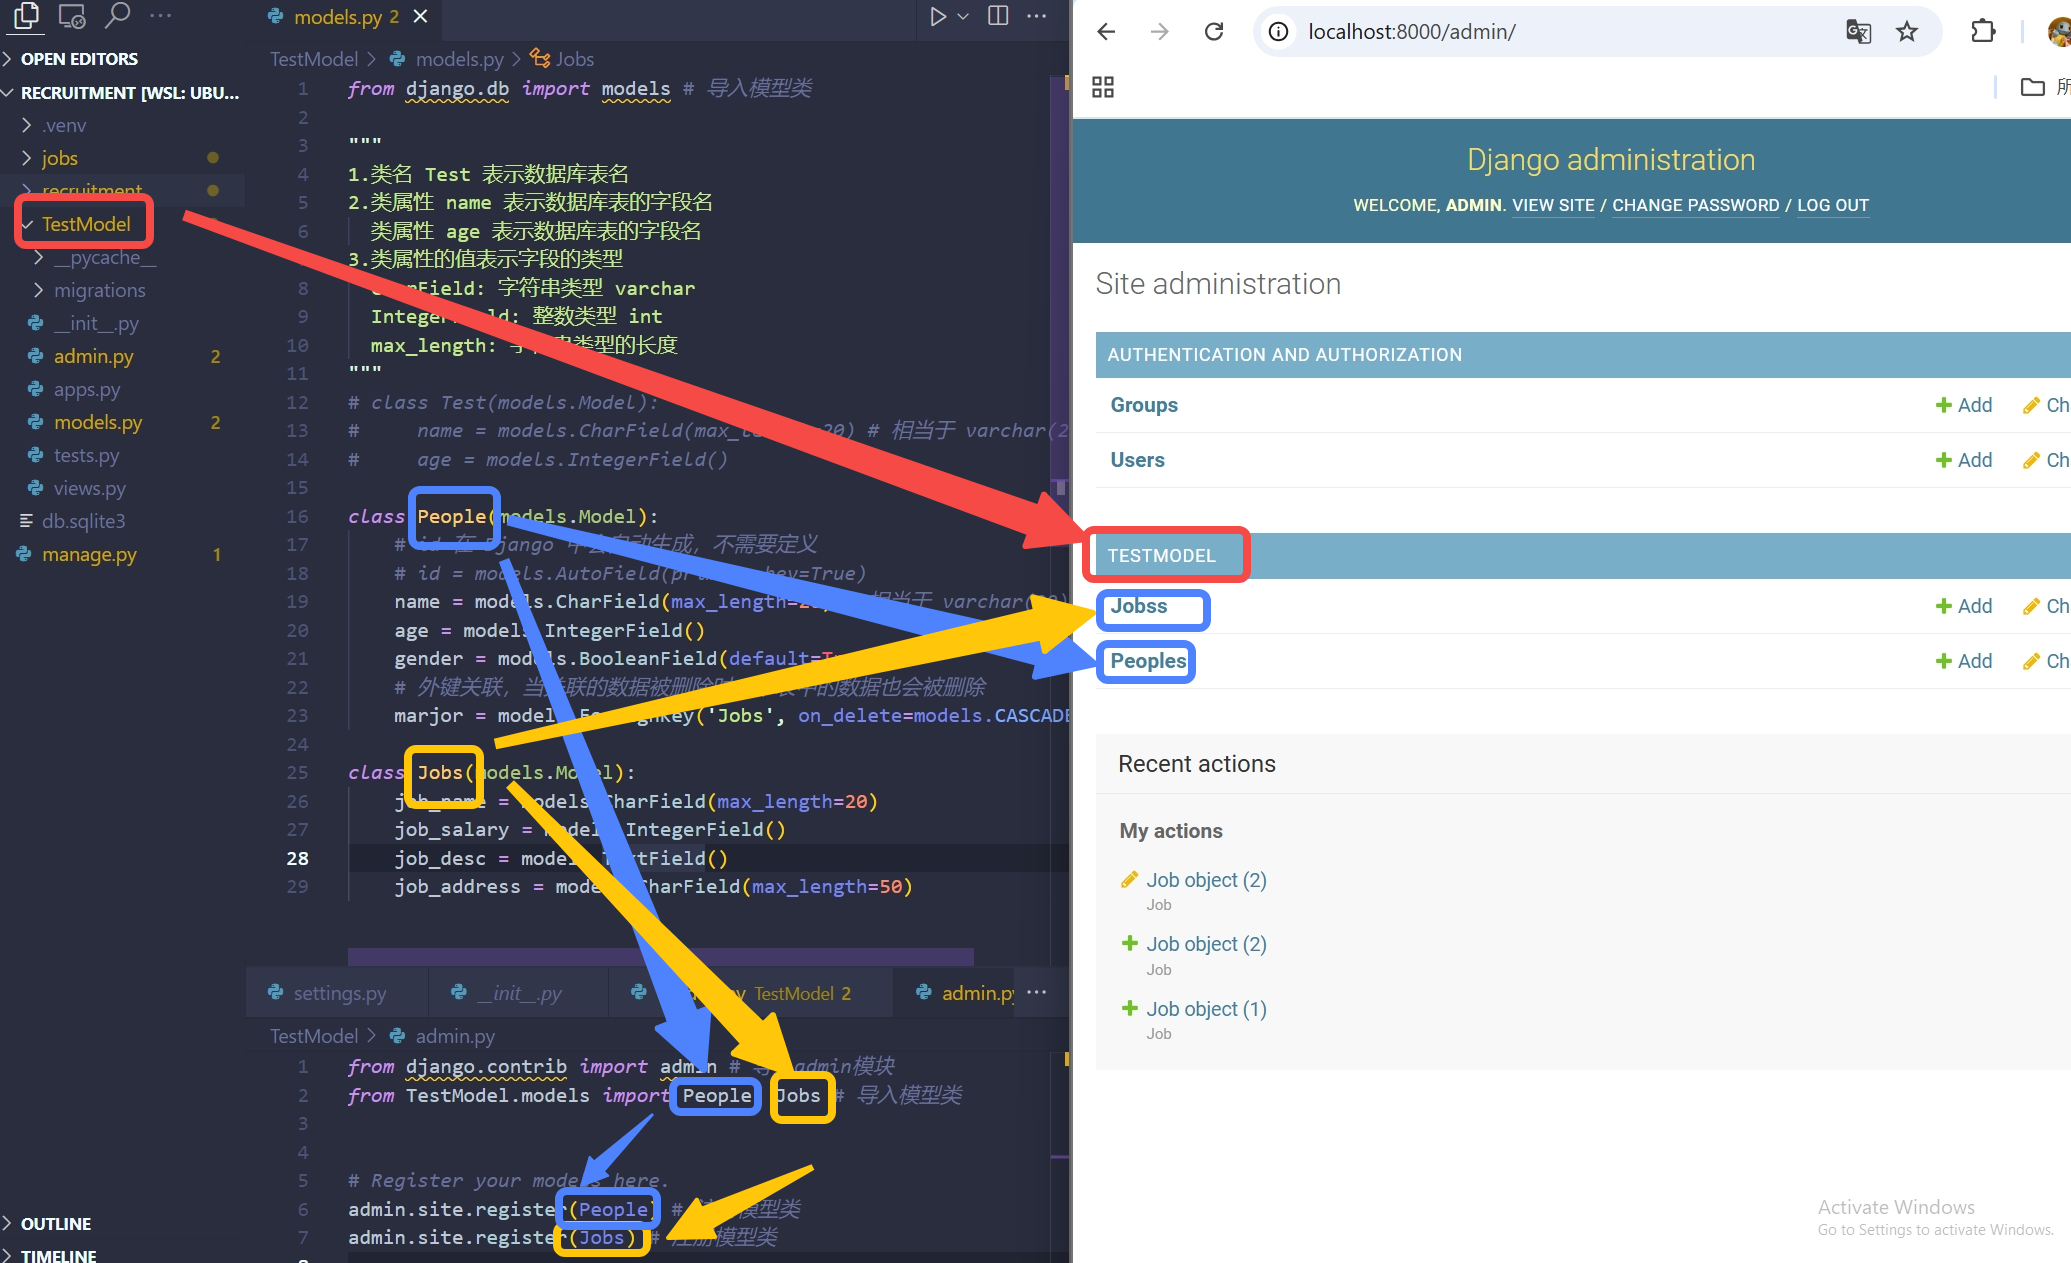
\includegraphics[width=0.6\textwidth]{part/互联/django/pic/模型/后台注册models.png}
    \caption{后台注册models}
    \label{fig:Django_后台注册models}
\end{figure}

如何对后台定义更多的信息，可以在模型类中设置\codeinline{Meta}类。
\begin{figure}[htpb]
    \centering
    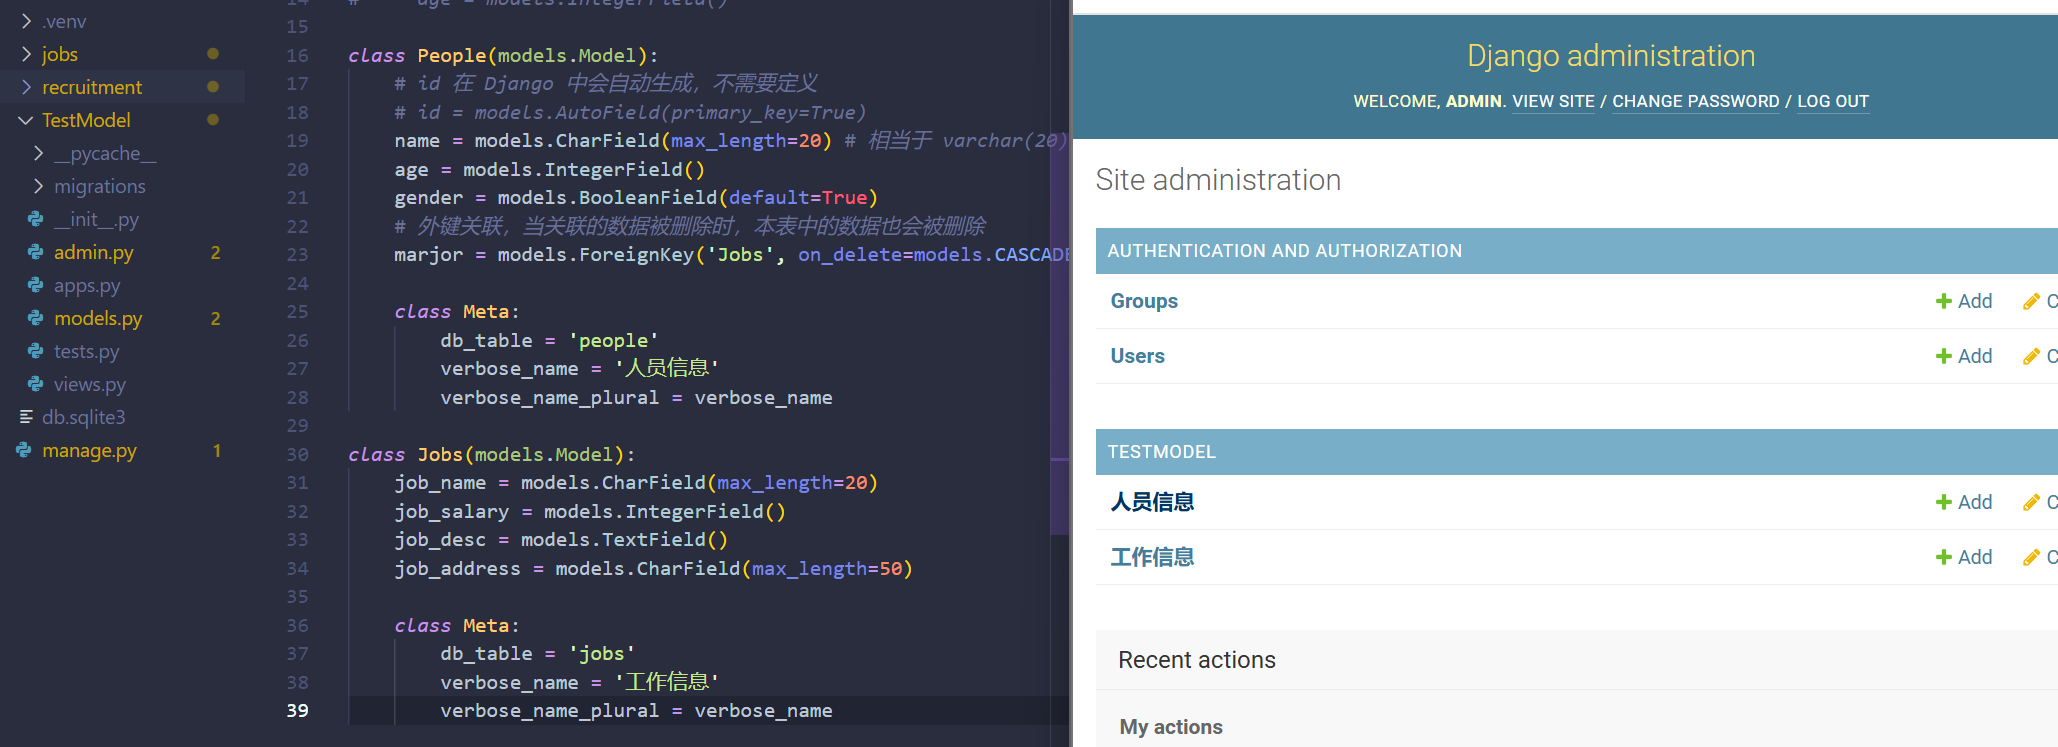
\includegraphics[width=0.6\textwidth]{part/互联/django/pic/模型/设置Meta信息.png}
    \caption{设置Meta信息}
    \label{fig:Django_设置Meta信息}
\end{figure}

如果想要在后台管理页面中显示更多的字段，可以在模型类中设置\codeinline{\_\_str\_\_()}方法。

如果想修改子应用在后台的名称，在子应用的\codeinline{apps.py}文件中设置\codeinline{verbose\_name}，如图\ref{fig:Django_修改子应用在后台的名称}所示。
\begin{lstlisting}[style=demostyle,numbers=none]
$> cat TestModel/apps.py
from django.apps import AppConfig


class TestmodelConfig(AppConfig):
    name = 'TestModel'
    verbose_name = '测试模型'

$> cat mysite/settings.py    
INSTALLED_APPS = [
    'django.contrib.admin',
    'django.contrib.auth',
    'django.contrib.contenttypes',
    'django.contrib.sessions',
    'django.contrib.messages',
    'django.contrib.staticfiles',
    # 'TestModel', # 添加创建的 app
    'TestModel.apps.TestmodelConfig', # 添加创建的 app
]
\end{lstlisting}
    
\begin{figure}[htpb]
    \centering
    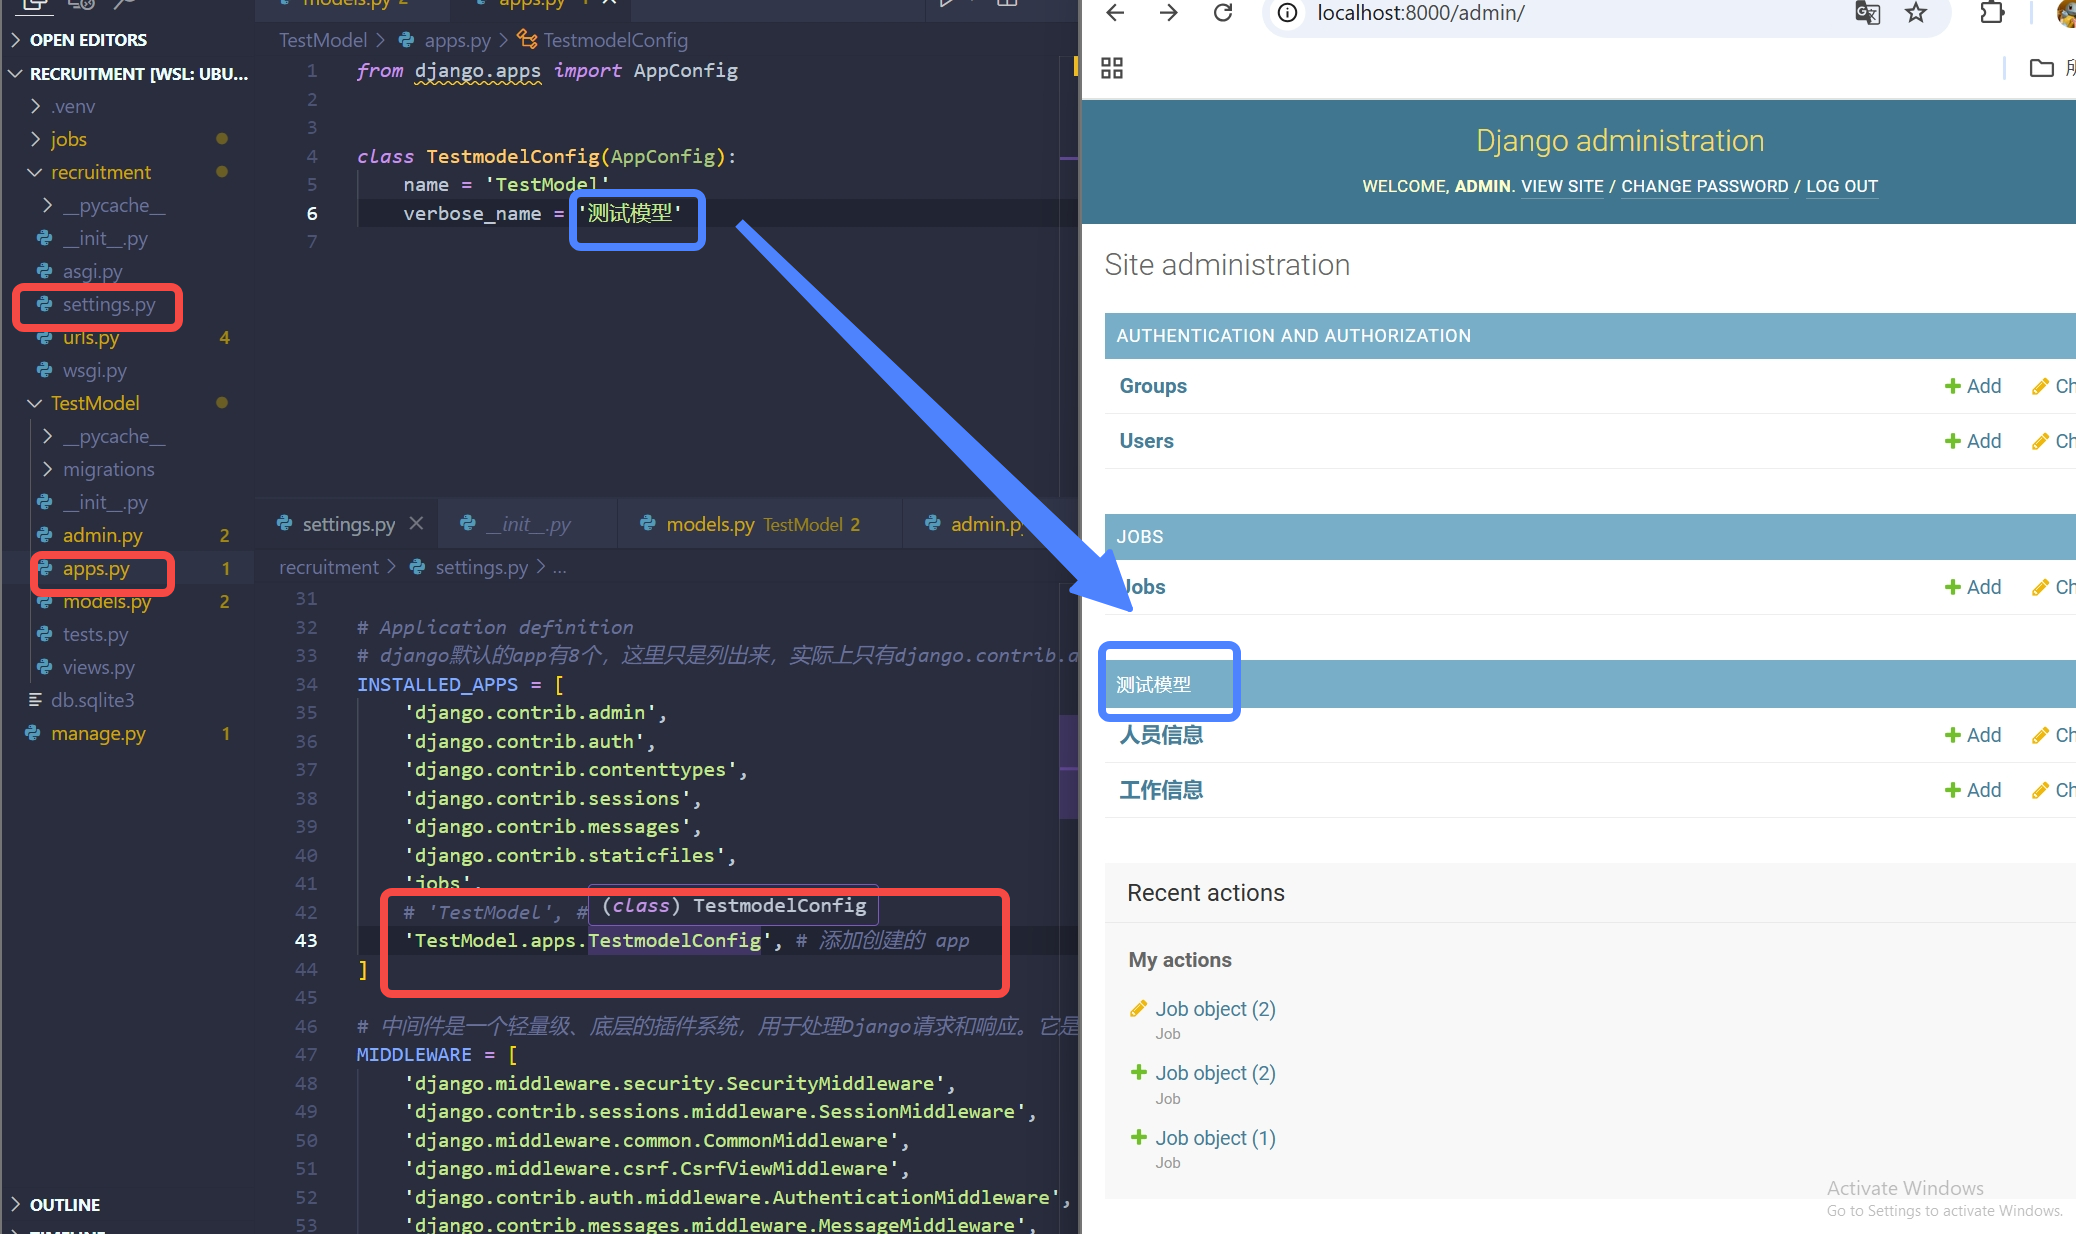
\includegraphics[width=0.6\textwidth]{part/互联/django/pic/模型/修改子应用在后台的名称.png}
    \caption{修改子应用在后台的名称}
    \label{fig:Django_修改子应用在后台的名称}
\end{figure}


\subsection{问题}
出现点击图\ref{fig:Django_设置Meta信息}中的子项出现404问题，解决方法如下：
\begin{figure}[htpb]
    \centering
    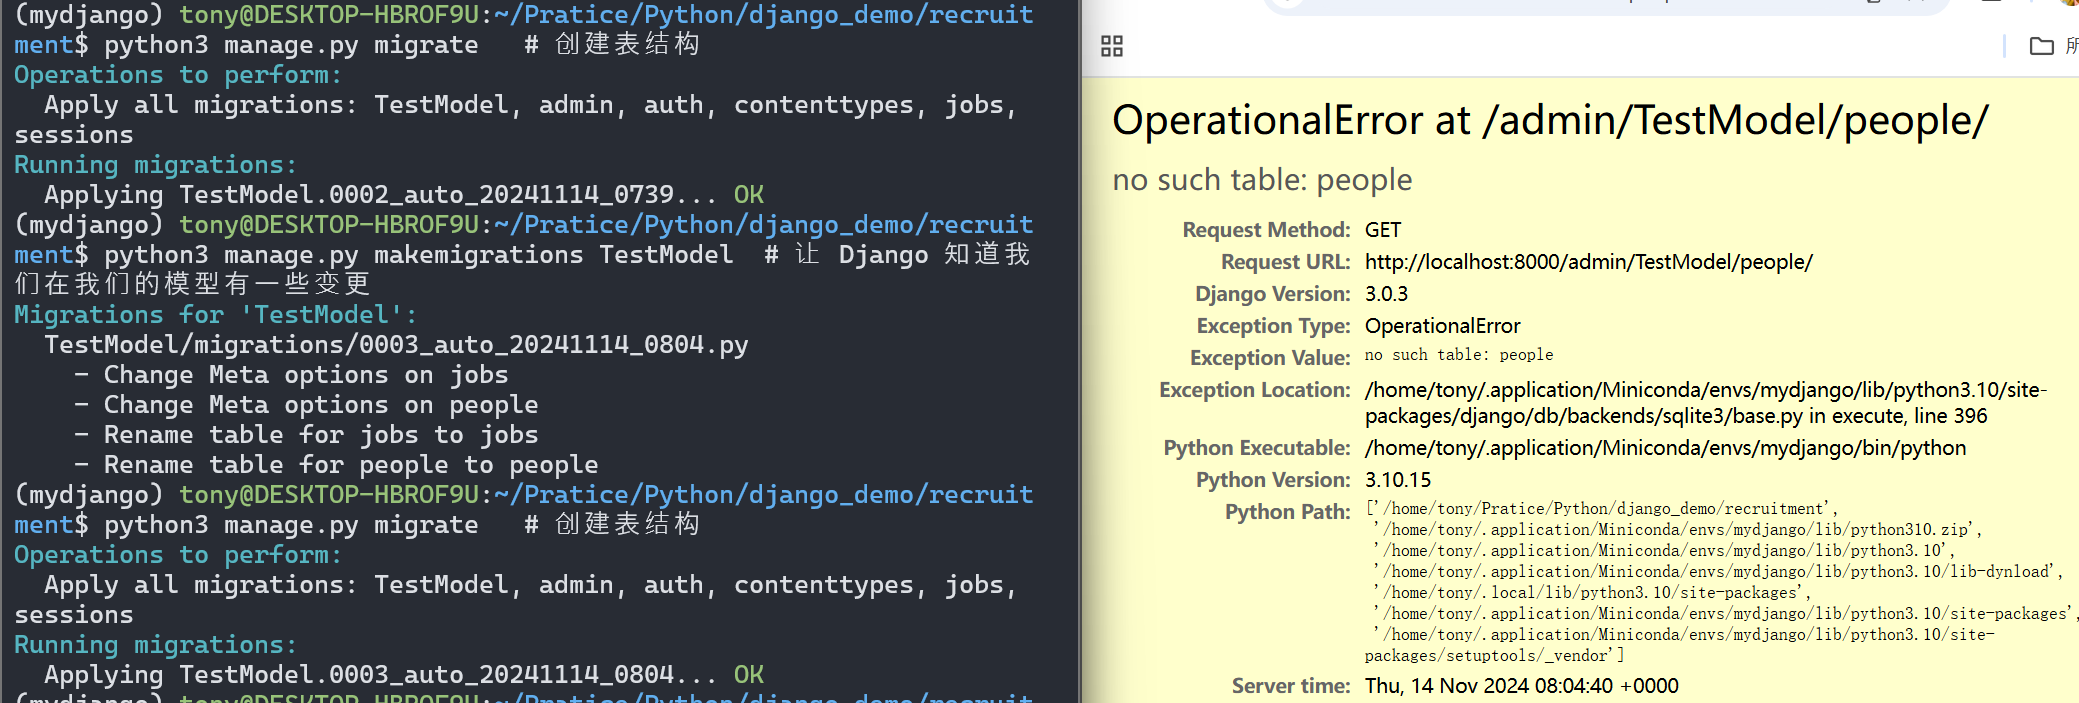
\includegraphics[width=0.4\textwidth]{part/互联/django/pic/模型/点击子项出现404问题.png}
    \caption{caption}
    \label{fig:label}
\end{figure}
\begin{lstlisting}[style=demostyle,numbers=none]
$ python3 manage.py makemigrations TestModel  # 让 Django 知道我们在我们的模型有一些变更
Migrations for 'TestModel':
  TestModel/migrations/0003_auto_20241114_0804.py
    - Change Meta options on jobs
    - Change Meta options on people
    - Rename table for jobs to jobs
    - Rename table for people to people

$ python3 manage.py migrate   # 创建表结构
Operations to perform:
  Apply all migrations: TestModel, admin, auth, contenttypes, jobs, sessions
Running migrations:
  Applying TestModel.0003_auto_20241114_0804... OK
\end{lstlisting}



